\documentclass[a4paper,10pt]{article}
\usepackage[T1]{fontenc}
\usepackage[utf8]{inputenc}
\usepackage[english]{babel}
\usepackage{lmodern}
\usepackage[top=1.6cm,bottom=1.8cm,left=1.9cm,right=1.9cm]{geometry}
\usepackage{titlesec,enumitem,xcolor,graphicx,lastpage,fancyhdr}
\usepackage{fontawesome5}
\usepackage[hidelinks]{hyperref}

\hypersetup{colorlinks=true,urlcolor=blue!70!black,linkcolor=blue!70!black}
\pagestyle{fancy}\fancyhf{}\renewcommand{\headrulewidth}{0pt}
\fancyfoot[C]{\small\color{gray}Page \thepage\ of \pageref{LastPage}}
\setlength{\parindent}{0pt}

\titleformat{\section}{\large\bfseries\color{blue!70!black}}{}{0em}{}[\vspace{-0.7em}\rule{\textwidth}{0.5pt}]
\titlespacing{\section}{0pt}{9pt}{5pt}
\setlist[itemize]{leftmargin=1.1em,itemsep=2pt,topsep=2pt,parsep=0pt}
\newcommand{\role}[4]{\vspace{3pt}\noindent\hspace{0.6em}\parbox[t]{0.38\textwidth}{\raggedright\textbf{#1}}\hfill\parbox[t]{0.58\textwidth}{\raggedleft\textit{#2}}\\{\textit{#3}\hfill\textit{#4}}\vspace{1pt}}

\begin{document}
\noindent
\begin{minipage}[t]{0.78\textwidth}
\vspace{0pt}
{\huge\bfseries Prabhavit Gupta}\\[8pt]
{\small \faPhone\ +39-351-610-7807 \quad \faEnvelope\ \href{mailto:prabhavitg@gmail.com}{prabhavitg@gmail.com} \quad \faLinkedin\ \href{https://www.linkedin.com/in/prabhavit/}{Linkedin} \quad \faMapMarker*\ Venice, Italy}
\end{minipage}\hfill
\begin{minipage}[t]{0.18\textwidth}
\vspace{0pt}\raggedleft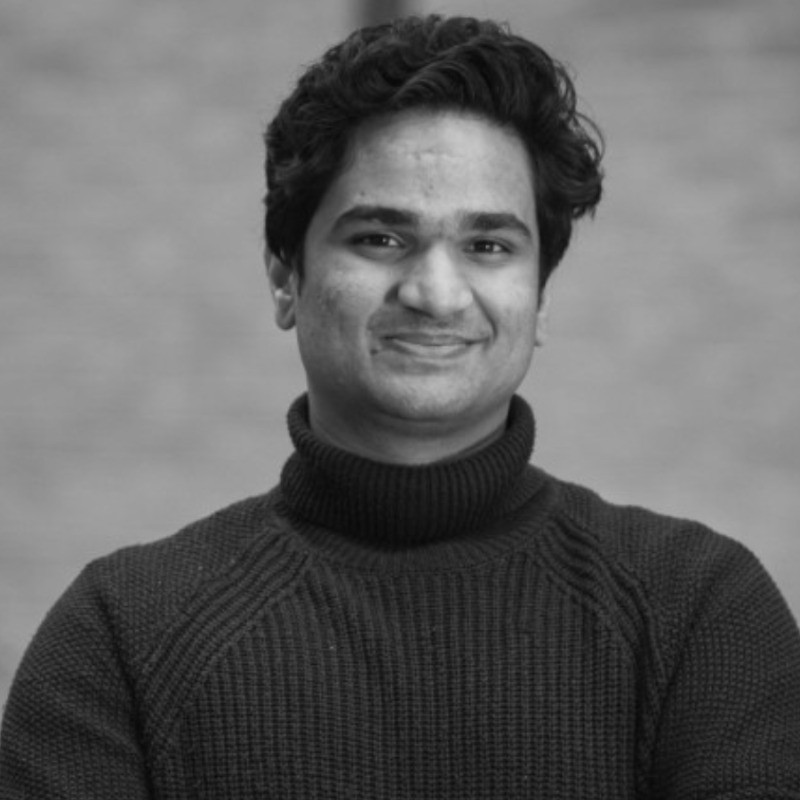
\includegraphics[width=2.3cm,height=2.3cm,keepaspectratio]{photo.jpg}
\end{minipage}

\section{Career Summary}
\begin{itemize}
\item IT Infrastructure \& Systems Automation Engineer with dual degrees in Mechanical Engineering and Management Engineering (Politecnico di Milano).
\item Experienced in administering Linux and Windows environments, virtualized infrastructure (Proxmox, Docker, VMs), and network operations across distributed sites.
\item Proficient in process automation and workflow orchestration using Python, Bash, n8n, SQL/MySQL, and Elasticsearch/ELK telemetry.
\item Skilled in bridging enterprise IT systems with industrial automation (PLC data acquisition, IoT sensors, Modbus/Ethernet protocols), supporting cross-border teams across Europe.
\end{itemize}

\section{Technical Skills}
\begin{itemize}
\item \textbf{IT Infrastructure \& Virtualization} -- Linux (Debian, Ubuntu, RHEL), Windows Server, Proxmox VE, KVM, Docker, Hyper-V, Network Administration (LAN/WAN, DNS, DHCP, VLAN, VPN)
\item \textbf{Scripting \& Automation} -- Python, Bash, n8n Workflows, PowerShell, REST APIs, Webhooks, Cron/Task Schedulers
\item \textbf{Data \& Observability} -- MySQL, PostgreSQL, Elasticsearch (Elastic Stack), Logstash, Kibana, Time-Series Logging, Grafana
\item \textbf{Industrial Integration \& IoT} -- PLC/SCADA Interfaces, Industrial IoT Sensors, Modbus, MQTT, OPC UA, Hardware-IT Gateways
\item \textbf{Support \& Tools} -- User Support, Fleet \& Hardware Management, Git, CI/CD, Jira, System Backup \& Disaster Recovery
\end{itemize}

\section{Visa \& Language}
\begin{itemize}
\item \textbf{Language} -- English (Fluent / Professional), Italian (Conversational / Intermediate), Hindi (Native), Spanish (Basic)
\item \textbf{Work Authorization} -- European Long Term Residence Permit (No Visa Sponsorship required). Driving License (Patente B). Available for travel.
\end{itemize}

\section{Professional Experience}
\role{\href{https://flowspace.co}{FlowSpace.co}}{IT Infrastructure \& Automation Lead}{London, UK / Remote}{Mar 2024 -- Ongoing}
\begin{itemize}
\item \textbf{Infrastructure Administration \& Virtualization:}
\begin{itemize}[label=--]
\item Administered hybrid Linux/Windows server environments and virtualized clusters (Proxmox, containerized microservices), maintaining 99.9\% system uptime.
\item Configured and secured site-to-site VPNs, network interfaces, DNS, and automated snapshot backup routines for disaster recovery.
\item Managed fleet provisioning, user access control, remote diagnostic support, and operational troubleshooting for international stakeholders.
\end{itemize}
\item \textbf{Automation \& Workflow Engineering:}
\begin{itemize}[label=--]
\item Developed Python automation scripts and n8n integration pipelines connecting internal databases, REST endpoints, and automated alerting services.
\item Built centralized logging and observability pipelines using Elasticsearch and MySQL to track infrastructure health and job queues.
\item Coordinated cross-functional IT operations with remote engineering teams across the UK and Europe.
\end{itemize}
\item \textit{Tools: Linux, Windows, Proxmox, Python, n8n, MySQL, Elastic, Docker, Bash, Git}
\end{itemize}

\role{Urlink}{Systems Automation Engineer}{Milan, Italy}{Jul 2023 -- Feb 2024}
\begin{itemize}
\item Implemented automated data pipelines linking industrial field equipment (PLCs, environmental sensors, IoT gateways) with central IT databases.
\item Handled on-site IT hardware configuration, network cabling, device provisioning, and end-user technical support for industrial clients.
\item Monitored relational database performance (MySQL) and automated daily backup verification routines.
\end{itemize}

\role{UltraStrategy}{IT \& Systems Automation Specialist}{Remote, Germany}{Sep 2022 -- Jun 2023}
\begin{itemize}
\item Developed Python and shell automation scripts for recurring sysadmin tasks, system diagnostics, and reporting.
\item Maintained virtual development environments and assisted with cross-site network and application troubleshooting.
\end{itemize}

\section{Education}
\role{Politecnico di Milano}{M.Sc. in Management Engineering (Digital Business \& ICT)}{Milan, Italy}{2020 -- 2023}
\role{Thapar Institute of Engineering and Technology}{B.E. in Mechanical Engineering}{Punjab, India}{2014 -- 2018}

\end{document}
